\documentclass[11pt]{article}
\usepackage{techcon_LaTeX_style}
\usepackage{comment}
\usepackage{hyperref}
\begin{document}

% ---------------
% NOTE: Do not change any of the LaTeX commands in this file unless
%       you really know what you are doing.  Further, any changes you
%       make must meet the Tech Con abstract guidelines
% ---------------


\tctitle{
SHARP: A Framework for Reproducible Benchmarking
}

\tcauthor{Eitan Frachtenberg, Pedro Bruel, Dejan Milojicic}
\tcbusinessgroup{Hewlett Packard Labs}
\tcemail{firstname.lastname@hpe.com}

\tcauthor{Gallig Renaud}
\tcbusinessgroup{GreenLake}
\tcemail{firstname.lastname@hpe.com}

\section*{Acknowledgements}

We Thank Viyom Mittal, Tobias Pfandzelter, Gourav Rattihalli, Aditya Dhakal, Rolando Pablo Hong Enriquez, and Ninad Hogade for their feedback and suggestions.

\newpage

\tctitle{
SHARP: A Framework for Reproducible Benchmarking
}

\tcabstract{
\textit{
Accurate performance measurement of computer systems is an art and a science. Many variables combine to add noise and uncertainty to performance measurements, such as architectural features (varying clock speeds, speculative execution, dynamic cache effects, etc.), use of accelerators, operating system decisions, workload and workflow variability, and even environmental factors.
Performance evaluation is even more challenging in modern scale-out computing such as HPC and GreenLake cluster, adding more variables and more heterogeneous components that increase performance variability.
The emergence of heterogeneous serverless computing (HSC) further complicates the performance picture with fine-grained computations that can vary in performance by many factors across consecutive runs.  
these trends lead to a difficult technical question: How do you evaluate the performance of the underlying platform effectively, accurately, and reproducibly?
The common methods of obtaining system performance, such as running a benchmark a few times and averaging the metrics, are inadequate. They can lead to results that are incomplete at best and misleading at worse. 
To address this gap, we introduce a framework and collection of tools called SHARP (``Serverless Heterogeneous Architecture Reproducible Performance''). SHARP augments existing benchmarks by introducing statistical rigor both to the performance measurement process and to the analysis of its products. In this paper, we review SHARP's design principles and discuss how it can produce (and reproduce) an accurate evaluation of all salient performance aspects of a given HSC, HPC, or cloud platform, including the hardware, the serverless framework, and the communication and I/O layers.
}
}


\section*{Problem statement}

Reproducibility is a cornerstone of technical progress because no experimental result can be fully established unless it can be independently reproduced~\cite{feitelson06:experimental}.
In particular, performance evaluation of computer systems is notoriously difficult to reproduce because of the myriad assumptions, underlying components, and methodological decisions that can affect performance, requiring detailed understanding and documentation of the system-under-test (SUT) to reproduce results~\cite{collberg16:repeatability, vitek11:repeatability}.
This task is complicated further when our evaluated system is running in the cloud~\cite{papadopoulos19:methodological}, and even further when we add serverless or heterogeneous computing, the focus of this work~\cite{garland13:determinism, hocko10:reducing}.
Sources of nondeterministic performance range from architecture (e.g., proprietary speculative execution algorithms), to operating systems and middleware (e.g., context switches), workloads (e.g., background jobs), benchmarks (e.g., randomized algorithms and Monte-Carlo simulations), and even the environment (e.g., datacenter temperature affecting CPU throttling)~\cite{cappello10:communication, gonnord23:survey, papadopoulos19:methodological}.
Consequently, benchmarks that produce performance summaries subject to these combined random variables can create an incomplete or inaccurate characterization of the system's performance~\cite{chiang13:determinism}.

This paper's starting point is that paradigms of heterogeneous, scale-out, and serverless computing carries potential performance and efficiency benefits.
But in order to verify these performance benefits, we must be able to accurately measure, report, and reproduce them.
An accurate and reproducible benchmarking framework could have direct business impact, such as comparing our supercomputers' performance to Cirrus and GreenLake; delivering solutions with consistent and convincing performance; evaluation of existing platforms and applications from other vendors; debugging and tuning performance in our products; and development of new hardware, software, and workflow offerings. %To this end, we must overcome two challenges:
The purpose of SHARP is to automate the correct measurement and analysis of performance benchmarks, as described next.

\begin{comment}

We address this gap by automating not only the production of detailed descriptions of the SUT and the benchmark execution, but also the embedding of source code and runtime parameters for both the measurements and the analysis in the reported results.
These details are automatically included in every run, allowing anyone to reproduce, enhance, and correct others' results with minimal configuration.

Another reproducibility challenge stems from noise.
Empirical measurements in computer systems, like all experiments of physical systems, ordinarily involve an element of noise: a variation in measurements that cannot be explained by controlled variations in the SUT
Noise hinders reproducible experimentation because it obscures the interpretation of diverging results: is the divergence due to a material difference in the SUT, or is it primarily within the noise?
In computer systems, this noise can emanate from the underlying hardware, the operating system, or the evaluated software itself.
These sources can be carefully observed, measured, and controlled to minimize some of the noise, but noise can never be fully eliminated, challenging reproducible benchmarking.

Instead of eliminating noise, another common approach to handling noise---which we incorporated holistically into SHARP---is to control for noise using statistical tools.
These tools include primarily the quantification of noise (by plotting of distributions of measurements, computing confidence intervals, etc.) and hypothesis testing (via computation of appropriate statistical tests and p-values).
Both of these approaches require some threshold amount of experimental repetition to produce a statistically meaningful treatment of noise.
The management of repetitions and the computation of noise statistics are all incorporated and automated in the SHARP framework.
\end{comment}

\section*{Our solution}

The guiding philosophy behind SHARP's design is that performance today should be treated as a distribution, not a number.
In other words, the goal of the performance evaluation should not be to approximate some performance summaries, such as mean throughput or $95^{th}$-percentile latency, because any such number fails to capture the rich variability of performance, and is therefore irreproducible and possibly misleading.
Instead, the goal should be to capture the distribution or statistical properties of performance, in a way that can reliably explain the variance from one test to the next and explain a wider range of likely outcomes.

To accomplish this goal, SHARP relies on three design principles: (1) distributions must be measured accurately; (2) distributions must be recorded completely, including their experimental conditions; and (3) distributions must be analyzed and clearly reported with statistical rigor.
SHARP itself is therefore not a benchmark, but a framework that runs benchmarks on diverse platforms to produce reproducible distributions.
Its architecture, shown in Figure~\ref{fig:architecture}, consists of modular components that facilitate this task.
Let us explore these components in greater detail.

\begin{figure}[ht]
\begin{center}
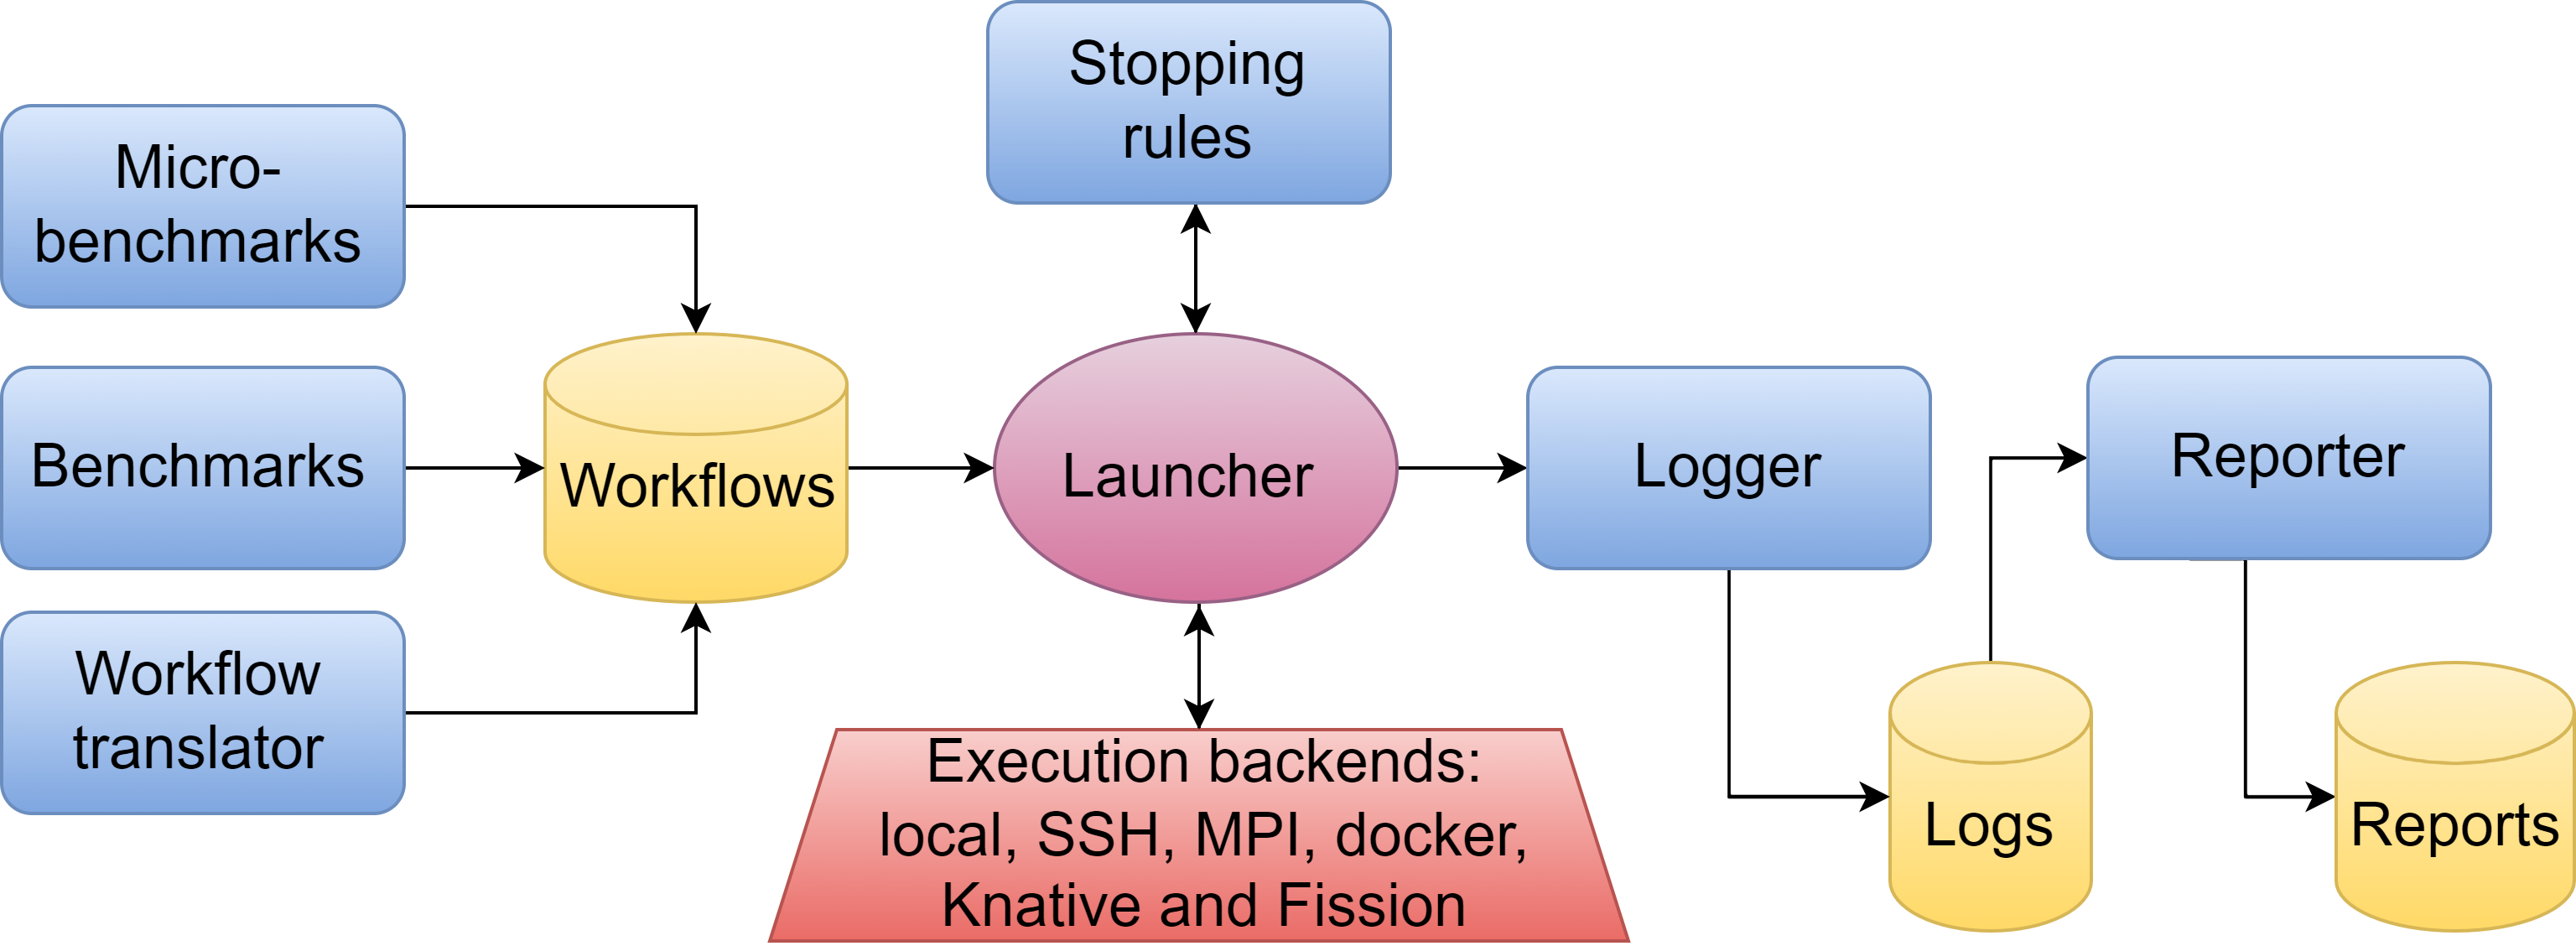
\includegraphics[height=1.5in]{architecture.png}
\caption{SHARP architecture}

\label{fig:architecture}
\end{center}
\end{figure}

\textbf{1) Workflows:}
SHARP was designed to run either microbenchmarks that focus on individual aspects of the system's performance (e.g., I/O or MPI synchronization), or complete benchmarks that focus on application performance (e.g., Linpack).
In the serverless parlance, we call these executable units ``functions''.
SHARP includes eleven such atomic and stateless functions, each representing a microbenchmark to measure a focused performance aspect, such as function invocation latency, SUT load response and saturation point, acccelerator performance, or MPI execution overhead. 
SHARP also includes functions to run a few open-source benchmarks, such as the Rodinia HPC suite and the GROMACS molecular dynamics benchmarks.

Modern workflows often combine different applications or application stages, sometimes with complicates dependency relationships.
To run these more complex workflows, we need to parse a workflow definition file and  execute its functions in order, both sequentially and in parallel, based on the direct-acyclic graph (DAG) of their dependencies.
Note that the successful completion of any workflow function is recorded via log files by the Logger module, and that Linux already includes a time-tested tool to execute a DAG based on file outputs, called `make'.
we therefore use `make` as the primary workflow definition file format for SHARP.
However, many competing formats exist with varying degrees of adoption but with similar information.
SHARP includes a standalone script to translate workflows from
a subset of the CNCF's open-standard \href{https://serverlessworkflow.github.io/}{Serverless Workflow Specification} (in JSON or YAML format) to a valid Makefile, which can then be run and rerun using `make'.


\textbf{2) Stopping rules:}
One of the key challenges in benchmarking is deciding on the appropriate number of samples (repeated measurements) to collect.
Choose too few, and the measurements would be unreliable; choose too many, and precious compute resources would be wasted; choose a wrong methodology, and the computations would be statistically unstable or invalid.
However, each benchmark and performance metric exhibits different distribution, so there is no one-size-fits-all rule for number of samples.
SHARP includes seven stopping rules tailored for specific types of distributions, such as lognormal.
It also includes a novel meta-heuristic to identify the most appropriate stopping rule for the dynamically observed distribution, so no prior knowledge is required to derive a statistically justifiable sample size.
We elaborate on this innovation in a parallel TechCon submission.

\textbf{3) Logger:}
A separate module automates the chore of logging all the performance data, independently of the function or platform.
All metrics are logged in a ``tidy data'' CSV file to facilitate statistical processing.
An accompanying markdown description file is automatically written alongside the raw data, describing each field in detail, as well as all the metadata required to recreate the SUT, including the current `git` hash of SHARP's own code.

\textbf{4) Launcher:}
The load generator---or launcher---is SHARP's centerpiece.
It executes individual functions or programs as prescribed by the workload whilst coordinating the execution backend, the stopping criteria, and the logging.
Launcher is a hierarchical, object-oriented class, with a specialization for every platform (backend) to run on, whether as a local process, remote process (via MPI or SSH), or a FaaS invocation (via shell commands or REST APIs that can leverage existing web load generators).
The behavior is the launcher is controlled from Make via the command line and is highly customizable.
Controls include repetition options and stopping criteria, cold and warm function invocations, timeouts, logging and descriptive parameters, parallelism, and backend options.
A particularly useful control to customize is the performance metrics to collect, which can be defined via a simple JSON or YAML interface.
This dynamic mechanism allows the launcher to collect arbitrary metrics such as run time or power consumption from any function with no code changes.

\textbf{5) Reporter:}
The final stage of the benchmark is the statistical processing of the raw data and the human-friendly presentation of results, implemented in a separate Reporter moule.
It uses RMarkdown scripts with a library of common statistical utilities for the analysis and reporting of distributions.
Executing these scripts on the CSV files that resulted from the workflow execution computes the desired performance metrics, as well as a suite of statistics to quantify uncertainty: means, medians, standard deviations, p-values, confidence intervals, statistical power, and hypothesis testing.
The metrics are also graphed and uncertainty measures across repetitive function copies are included as either confidence intervals or graphical distribution descriptions.
% Fig. \ref{fig:perfexample} exemplifies two performance metrics computed by SHARP with different visualizations of uncertainty.
The resulting reports can be exported to PDF, Word, LaTeX, HTML, or Powerpoint format.
The execution of the markdown files is delegated to a Docker container that freezes all of the statistical and graphing software prerequisites to facilitate reproduction of the reports.
Any change in the underlying platform, software, hardware, or even just time passed can be captured by simply rerunning the workflow and reporting.
The resulting report includes all of the graphics, statistics, and descriptive narratives.
The conclusion part of the report must still be added manually---SHARP reliably automates performance measurement, but leaves its interpretation to humans.


\section*{Evidence the solution works}

%Provide either results from end users of the solution
%demonstrating that you effectively
%addressed the original problem,
%or other convincing
%demonstrations that the proposal has substantiated merit. 

- Integration with Autobench
- Usage in performance prediction
- Show a snazzy graph.

\section*{Competitive approaches}

With the recent emergence of serverless computing, a number of benchmarks and microbenchmarks have been proposed as well~\cite{copik21:sebs, decker22:performance, hancock22:orcbench, kim19:practical, yu20:characterizing}.
Since all of these benchmarks were designed for homogeneous FaaS platforms, they are not directly comparable.
Similarly, a number of benchmarks exist for heterogeneous architectures, but they do not employ the serverless model~\cite{danalis10:scalable}.
We also note that while many of these benchmarks compute sophisticated performance metrics, none emphasizes reproducibility in reporting and analysis as ours does~\cite{scheuner20:review}, following the eight principles of reproducible cloud performance evaluation laid out by Papadopoulos et al.~\cite{papadopoulos19:methodological}.
One more crucial difference is that we also plan to analyze energy consumption and efficiency via metrics collected directly from iLO, as well as a collection of complex real applications and workflows.



\section*{Current status and Next steps}

The current, version of SHARP reliably and reproducibly answers descriptive performance questions such as ``what is the performance of application X on system Y? How does it vary? How confident can we be in these numbers?''.
These are useful questions to answer in today's increasingly complex HPC and heterogeneous systems, where performance becomes increasingly hard to describe with a single number or two.
SHARP has already successfully integrated with GreenLake's AutoBench, and is currently being used in a large-scale effort to right-size GreenLake cloud modules (see related submission).

The next development phase envisions a move towards explainable performance, answering questions such as ``What system features explain variability for this function? Can we model and predict the performance variability under different assumptions?''
We also plan to incorporate Bayesian inference into our statistical toolkit to improve comparisons across time or machines and enable accurate performance regression testing.
Such features in turn will enable important business applications, such as fine-tuning latency-senstitive HPC and AI applications, optimization of power consumption, and informed decisions on future hardware to design, procure, or debug.

\newpage
\section*{References}

\bibliographystyle{plain}
\bibliography{hsc}  

\end{document}
